\documentclass{beamer}

\usepackage{epsfig,graphicx,parskip,setspace,tabularx,xspace,url,holtexbasic,alltt,proof,tikz}
\usetikzlibrary{arrows}
\usetikzlibrary{positioning}
\usetheme{CambridgeUS}

\title[Verified register allocation]{Developing a formally verified algorithm for register allocation}
\subtitle{A Part III project}
\author{David Barker}
\date{9\textsuperscript{th} June 2014}
\subject{Computer Science}


\begin{document}

\frame{\titlepage}

\section{Introduction}

\begin{frame}
\frametitle{Introduction}
\framesubtitle{The problem of register allocation}

\begin{itemize}
	\item Intermediate code assumes infinite registers, whilst real machines have finite registers
	\item Using memory costs many cycles
	\item When two variables are never used at the same time they can be stored in the same register
	\item Minimising register usage allows more data to be stored in registers
\end{itemize}
\end{frame}

\subsection{Register allocation by graph colouring}
\begin{frame}[containsverbatim]
\frametitle{Register allocation by graph colouring}
\framesubtitle{Computing live ranges}
\begin{center}
\begin{alltt}
R1 = R2 + R3  \textcolor{red}{\(\{R_2, R_3\}\)}
R4 = R1 * R2  \textcolor{red}{\(\{R_1, R_2, R_3\}\)}
R5 = R3 - R4  \textcolor{red}{\(\{R_1, R_3, R_4\}\)}
R6 = R1 + R5  \textcolor{red}{\(\{R_1, R_5\}\)}
\end{alltt}
\end{center}
\end{frame}

\begin{frame}[containsverbatim]
\frametitle{Building a clash graph}
\begin{columns}[c]
\column{.5\textwidth}
\begin{alltt}
R1 = R2 + R3  \(\{R_2, R_3\}\)
R4 = R1 * R2  \(\{R_1, R_2, R_3\}\)
R5 = R3 - R4  \(\{R_1, R_3, R_4\}\)
R6 = R1 + R5  \(\{R_1, R_5\}\)
\end{alltt}
\column{.5\textwidth}
\begin{figure}[!ht]
  \centering
  \includegraphics[width=0.8\textwidth]{graph.pdf}
\end{figure}
\end{columns}
\end{frame}

\begin{frame}
\frametitle{Colouring the clash graph}
\begin{columns}[c]
\column{.5\textwidth}
\begin{figure}[!ht]
  \centering
  \includegraphics[width=0.8\textwidth]{graph.pdf}
\end{figure}
\column{.5\textwidth}
\begin{figure}[!ht]
  \centering
  \includegraphics[width=0.8\textwidth]{colouredGraph.pdf}
\end{figure}
\end{columns}
\end{frame}

\begin{frame}[containsverbatim]
\frametitle{Applying the colouring}
\begin{columns}[c]
\column{.5\textwidth}
\begin{figure}[!ht]
  \centering
  \includegraphics[width=0.8\textwidth]{colouredGraph.pdf}
\end{figure}
\column{.5\textwidth}
\begin{alltt}
\textcolor{green}{R1} = \textcolor{blue}{R2} + \textcolor{red}{R3}
\textcolor{cyan}{R4} = \textcolor{green}{R1} * \textcolor{blue}{R2}
\textcolor{red}{R3} = \textcolor{red}{R3} - \textcolor{cyan}{R4}
\textcolor{cyan}{R4} = \textcolor{green}{R1} + \textcolor{red}{R3}
\end{alltt}
\end{columns}
\end{frame}

\begin{frame}
\frametitle{The full algorithm}

\begin{columns}[c]
\column{.5\textwidth}
 \begin{center}
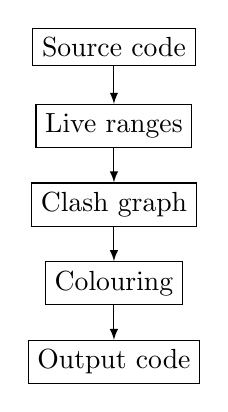
\begin{tikzpicture}[node distance = 1cm, auto]
    % Place nodes
    \node [draw] (source) {Source code};
    \node [draw, below of=source] (live) {Live ranges};
    \node [draw, below of=live] (graph) {Clash graph};
    \node [draw, below of=graph] (colouring) {Colouring};
    \node [draw, below of=colouring] (code) {Output code};
    % Draw edges
    \draw [-latex] (source) -- (live);
    \draw [-latex] (live) -- (graph);
    \draw [-latex] (graph) -- (colouring);
    \draw [-latex] (colouring) -- (code);
\end{tikzpicture}
\end{center}
\column{.5\textwidth}
 A correct algorithm will generate output code with exactly the same behaviour
\end{columns}
\end{frame}

\subsection{Guaranteeing correctness}
\begin{frame}[containsverbatim]
\frametitle{How we ensure this behaviour}
A correct algorithm produces a colouring which causes no conflicts between simultaneously live registers:

\begin{alltt}\small
	\HOLConst{colouring_ok_alt} \HOLFreeVar{c} \HOLFreeVar{code} \HOLFreeVar{live} \HOLTokenEquiv{}
\HOLConst{colouring_respects_conflicting_sets} \HOLFreeVar{c}
  (\HOLConst{conflicting_sets} \HOLFreeVar{code} \HOLFreeVar{live})
\end{alltt}

This was proved sufficient: a colouring satisfying this will always yield code with unchanged behaviour
\end{frame}

\section{Modelling the problem}
\begin{frame}[containsverbatim]
\frametitle{Code representation}
A block of code is represented by a list of three-address instructions:

\begin{alltt}\small
	\HOLTyOp{inst} = \HOLConst{Inst} \HOLKeyword{of} \HOLTyOp{num} \HOLTokenImp{} \HOLTyOp{num} \HOLTokenImp{} \HOLTyOp{num}
\end{alltt}

This is evaluated on a store $s$ as follows:

\begin{alltt}\small
	\HOLConst{eval} \HOLFreeVar{f} \HOLFreeVar{s} [] = \HOLFreeVar{s}
\HOLConst{eval} \HOLFreeVar{f} \HOLFreeVar{s} (\HOLConst{Inst} \HOLFreeVar{w} \HOLFreeVar{r\sb{\mathrm{1}}} \HOLFreeVar{r\sb{\mathrm{2}}}::\HOLFreeVar{code}) =
\HOLConst{eval} \HOLFreeVar{f} ((\HOLFreeVar{w} =+ \HOLFreeVar{f} (\HOLFreeVar{s} \HOLFreeVar{r\sb{\mathrm{1}}}) (\HOLFreeVar{s} \HOLFreeVar{r\sb{\mathrm{2}}})) \HOLFreeVar{s}) \HOLFreeVar{code}
\end{alltt}
\end{frame}

\begin{frame}[containsverbatim]
Colourings are functions of type $num \rightarrow num$

Colourings can be applied simply by substituting registers:

\begin{alltt}\small
	\HOLConst{apply} \HOLFreeVar{c} [] = []
\HOLConst{apply} \HOLFreeVar{c} (\HOLConst{Inst} \HOLFreeVar{w} \HOLFreeVar{r\sb{\mathrm{1}}} \HOLFreeVar{r\sb{\mathrm{2}}}::\HOLFreeVar{code}) =
\HOLConst{Inst} (\HOLFreeVar{c} \HOLFreeVar{w}) (\HOLFreeVar{c} \HOLFreeVar{r\sb{\mathrm{1}}}) (\HOLFreeVar{c} \HOLFreeVar{r\sb{\mathrm{2}}})::\HOLConst{apply} \HOLFreeVar{c} \HOLFreeVar{code}
\end{alltt}
\end{frame}

\begin{frame}[containsverbatim]
\frametitle{Set representation}
To simplify definitions and proofs, sets are represented as duplicate-free lists and all functions manipulating them are proven to preserve duplicate-freeness

Many simple set functions were implemented preserving this representation, for example:

\begin{alltt}\small
	\HOLConst{insert} \HOLFreeVar{x} \HOLFreeVar{xs} = \HOLKeyword{if} \HOLConst{MEM} \HOLFreeVar{x} \HOLFreeVar{xs} \HOLKeyword{then} \HOLFreeVar{xs} \HOLKeyword{else} \HOLFreeVar{x}::\HOLFreeVar{xs}
\end{alltt}

\begin{alltt}\small
	\HOLConst{delete} \HOLFreeVar{x} \HOLFreeVar{xs} = \HOLConst{FILTER} (\HOLTokenLambda{}\HOLBoundVar{y}. \HOLFreeVar{x} \HOLTokenNotEqual{} \HOLBoundVar{y}) \HOLFreeVar{xs}
\end{alltt}
\end{frame}

\section{The algorithm}
\subsection{Live variable analysis}

\begin{frame}[containsverbatim]
\frametitle{The algorithm}
\framesubtitle{Live variable analysis}
The set of live variables before a block of code is given by the following equation:

\begin{center}
$live(n) = \left(live(n+1) \setminus write(n)\right) \cup read(n)$
\end{center}

This was implemented as follows:

\begin{alltt}\small
	\HOLConst{get_live} [] \HOLFreeVar{live} = \HOLFreeVar{live}
\HOLConst{get_live} (\HOLConst{Inst} \HOLFreeVar{w} \HOLFreeVar{r\sb{\mathrm{1}}} \HOLFreeVar{r\sb{\mathrm{2}}}::\HOLFreeVar{code}) \HOLFreeVar{live} =
\HOLConst{insert} \HOLFreeVar{r\sb{\mathrm{1}}} (\HOLConst{insert} \HOLFreeVar{r\sb{\mathrm{2}}} (\HOLConst{delete} \HOLFreeVar{w} (\HOLConst{get_live} \HOLFreeVar{code} \HOLFreeVar{live})))
\end{alltt}
\end{frame}

\begin{frame}[containsverbatim]
\frametitle{Correctness}
This was implicitly proved correct as its usage led to an algorithm proven to generate behaviour-preserving colourings

More directly, it was proved that only registers returned by \texttt{get\_live} affect program behaviour:

\begin{alltt}\small
	\HOLTokenTurnstile{} (\HOLConst{MAP} \HOLFreeVar{s} (\HOLConst{get_live} \HOLFreeVar{code} \HOLFreeVar{live}) = \HOLConst{MAP} \HOLFreeVar{t} (\HOLConst{get_live} \HOLFreeVar{code} \HOLFreeVar{live})) \HOLTokenImp{}
   (\HOLConst{MAP} (\HOLConst{eval} \HOLFreeVar{f} \HOLFreeVar{s} \HOLFreeVar{code}) \HOLFreeVar{live} = \HOLConst{MAP} (\HOLConst{eval} \HOLFreeVar{f} \HOLFreeVar{t} \HOLFreeVar{code}) \HOLFreeVar{live})
\end{alltt}
\end{frame}

\subsection{Clash graph generation}
\begin{frame}
\frametitle{Clash graph generation}
\framesubtitle{Clash graph representation}
Graphs are represented as lists of (vertex, clash list) pairs, for example:

$[ (r_1, [c_1, \ldots, c_n]), \ldots, (r_n, [c_1, \ldots, c_n]) ]$

Here $r_n$ is the $n^{th}$ register and $c_n$ is the $n^{th}$ register conflicting with it.

This makes it simple to iterate over vertices, and the list can be re-ordered to prioritise certain vertices for colouring.
\end{frame}

\begin{frame}[containsverbatim]
\frametitle{Building the graph}
First we need to get the list of registers conflicting with a given register:

\begin{alltt}\small
	\HOLConst{conflicts_for_register} \HOLFreeVar{r} \HOLFreeVar{code} \HOLFreeVar{live} =
\HOLConst{delete} \HOLFreeVar{r}
  (\HOLConst{list_union_flatten}
     (\HOLConst{FILTER} (\HOLTokenLambda{}\HOLBoundVar{set}. \HOLConst{MEM} \HOLFreeVar{r} \HOLBoundVar{set}) (\HOLConst{conflicting_sets} \HOLFreeVar{code} \HOLFreeVar{live})))
\end{alltt}

This function is then used to build a graph in the specified format:

\begin{alltt}\small
	\HOLConst{get_conflicts} \HOLFreeVar{code} \HOLFreeVar{live} =
\HOLConst{MAP} (\HOLTokenLambda{}\HOLBoundVar{reg}. (\HOLBoundVar{reg},\HOLConst{conflicts_for_register} \HOLBoundVar{reg} \HOLFreeVar{code} \HOLFreeVar{live}))
  (\HOLConst{get_registers} \HOLFreeVar{code} \HOLFreeVar{live})
\end{alltt}
\end{frame}

\begin{frame}[containsverbatim]
\frametitle{Correctness of generated clash graphs}
Verification of the clash graph generation stage consisted of three main proofs:

\begin{itemize}
	\item Registers never conflict with themselves (follows easily from the definition of \texttt{conflicts\_for\_register})

	\begin{alltt}\small
		\HOLTokenTurnstile{} \HOLFreeVar{r} \HOLTokenNotIn{} \HOLConst{set} (\HOLConst{conflicts_for_register} \HOLFreeVar{r} \HOLFreeVar{code} \HOLFreeVar{live})
	\end{alltt}

	\item The graph is complete: any registers from the same conflicting set appear in each other's conflicts

	\begin{alltt}\small
		\HOLTokenTurnstile{} \HOLConst{MEM} \HOLFreeVar{c} (\HOLConst{conflicting_sets} \HOLFreeVar{code} \HOLFreeVar{live}) \HOLTokenConj{} \HOLConst{MEM} \HOLFreeVar{r} \HOLFreeVar{c} \HOLTokenConj{} \HOLConst{MEM} \HOLFreeVar{s} \HOLFreeVar{c} \HOLTokenConj{}
   \HOLFreeVar{r} \HOLTokenNotEqual{} \HOLFreeVar{s} \HOLTokenImp{}
   \HOLConst{MEM} \HOLFreeVar{r} (\HOLConst{conflicts_for_register} \HOLFreeVar{s} \HOLFreeVar{code} \HOLFreeVar{live})
	\end{alltt}
\end{itemize}
\end{frame}

\begin{frame}[containsverbatim]
\begin{itemize}
	\item The graph doesn't contain any false conflicts: every conflict is the result of two registers appearing in a conflicting set together

	\begin{alltt}\small
		\HOLTokenTurnstile{} \HOLConst{MEM} \HOLFreeVar{r\sb{\mathrm{1}}} (\HOLConst{conflicts_for_register} \HOLFreeVar{r\sb{\mathrm{2}}} \HOLFreeVar{code} \HOLFreeVar{live}) \HOLTokenImp{}
   \HOLTokenExists{}\HOLBoundVar{c}. \HOLConst{MEM} \HOLBoundVar{c} (\HOLConst{conflicting_sets} \HOLFreeVar{code} \HOLFreeVar{live}) \HOLTokenConj{} \HOLConst{MEM} \HOLFreeVar{r\sb{\mathrm{1}}} \HOLBoundVar{c} \HOLTokenConj{} \HOLConst{MEM} \HOLFreeVar{r\sb{\mathrm{2}}} \HOLBoundVar{c}
	\end{alltt}
\end{itemize}
\end{frame}

\subsection{Colouring algorithms}

\begin{frame}[containsverbatim]
\frametitle{Colouring algorithms}
\framesubtitle{Defining correctness}
A graph colouring is correct if no vertex has the same colour as any of its neighbours. This is captured in the definition below:

\begin{alltt}\small
	\HOLConst{colouring_satisfactory} \HOLFreeVar{col} [] \HOLTokenEquiv{} \HOLConst{T}
\HOLConst{colouring_satisfactory} \HOLFreeVar{col} ((\HOLFreeVar{r},\HOLFreeVar{rs})::\HOLFreeVar{cs}) \HOLTokenEquiv{}
\HOLFreeVar{col} \HOLFreeVar{r} \HOLTokenNotIn{} \HOLConst{set} (\HOLConst{MAP} \HOLFreeVar{col} \HOLFreeVar{rs}) \HOLTokenConj{} \HOLConst{colouring_satisfactory} \HOLFreeVar{col} \HOLFreeVar{cs}
\end{alltt}

This was shown to imply the earlier definition of colouring correctness:

\begin{alltt}\small
	\HOLTokenTurnstile{} \HOLConst{duplicate_free} \HOLFreeVar{live} \HOLTokenImp{}
   \HOLConst{colouring_satisfactory} \HOLFreeVar{c} (\HOLConst{get_conflicts} \HOLFreeVar{code} \HOLFreeVar{live}) \HOLTokenImp{}
   \HOLConst{colouring_ok_alt} \HOLFreeVar{c} \HOLFreeVar{code} \HOLFreeVar{live}
\end{alltt}

Thus proving that a colouring satisfies \texttt{colouring\_satisfactory} is sufficient to show that it preserves program behaviour
\end{frame}

\begin{frame}[containsverbatim]
\frametitle{Requirements on clash graphs}
For verification to work, it was necessary to show that generated graphs satisfy several properties:

\begin{itemize}
	\item Edge lists must contain no duplicates and vertices must not clash with themselves:
	
	\begin{alltt}\small
		\HOLConst{edge_list_well_formed} (\HOLFreeVar{v},\HOLFreeVar{edges}) \HOLTokenEquiv{}
\HOLFreeVar{v} \HOLTokenNotIn{} \HOLConst{set} \HOLFreeVar{edges} \HOLTokenConj{} \HOLConst{duplicate_free} \HOLFreeVar{edges}
	\end{alltt}
	
	\item Graphs must not contain duplicate vertices:
	
	\begin{alltt}\small
		\HOLConst{graph_duplicate_free} [] \HOLTokenEquiv{} \HOLConst{T}
\HOLConst{graph_duplicate_free} ((\HOLFreeVar{r},\HOLFreeVar{rs})::\HOLFreeVar{cs}) \HOLTokenEquiv{}
(\HOLTokenForall{}\HOLBoundVar{rs\sp{\prime}}. (\HOLFreeVar{r},\HOLBoundVar{rs\sp{\prime}}) \HOLTokenNotIn{} \HOLConst{set} \HOLFreeVar{cs}) \HOLTokenConj{} \HOLConst{graph_duplicate_free} \HOLFreeVar{cs}
	\end{alltt}
\end{itemize}
\end{frame}

\begin{frame}[containsverbatim]
\begin{itemize}
	\item Graphs must be symmetric -- if $v_1$ appears in the conflicts for $v_2$, $v_2$ appears in the conflicts for $v_1$:
	
	\begin{alltt}\small
		\HOLConst{graph_reflects_conflicts} \HOLFreeVar{cs} \HOLTokenEquiv{}
\HOLTokenForall{}\HOLBoundVar{r\sb{\mathrm{1}}} \HOLBoundVar{r\sb{\mathrm{2}}} \HOLBoundVar{rs\sb{\mathrm{1}}} \HOLBoundVar{rs\sb{\mathrm{2}}}.
  \HOLConst{MEM} (\HOLBoundVar{r\sb{\mathrm{1}}},\HOLBoundVar{rs\sb{\mathrm{1}}}) \HOLFreeVar{cs} \HOLTokenConj{} \HOLConst{MEM} (\HOLBoundVar{r\sb{\mathrm{2}}},\HOLBoundVar{rs\sb{\mathrm{2}}}) \HOLFreeVar{cs} \HOLTokenConj{} \HOLConst{MEM} \HOLBoundVar{r\sb{\mathrm{1}}} \HOLBoundVar{rs\sb{\mathrm{2}}} \HOLTokenImp{} \HOLConst{MEM} \HOLBoundVar{r\sb{\mathrm{2}}} \HOLBoundVar{rs\sb{\mathrm{1}}}
	\end{alltt}
\end{itemize}

These were all proven to hold of the graphs generated by the clash graph step
\end{frame}

\begin{frame}[containsverbatim]
\frametitle{Verified colouring algorithms}
The first colouring algorithm verified was a naive one which simply assigns a new colour to each vertex:

\begin{alltt}\small
	\HOLConst{naive_colouring_aux} [] \HOLFreeVar{n} = (\HOLTokenLambda{}\HOLBoundVar{x}. \HOLFreeVar{n})
\HOLConst{naive_colouring_aux} ((\HOLFreeVar{r},\HOLFreeVar{rs})::\HOLFreeVar{cs}) \HOLFreeVar{n} =
(\HOLFreeVar{r} =+ \HOLFreeVar{n}) (\HOLConst{naive_colouring_aux} \HOLFreeVar{cs} (\HOLFreeVar{n} + 1))
\end{alltt}

\begin{alltt}\small
	\HOLConst{naive_colouring} \HOLFreeVar{constraints} = \HOLConst{naive_colouring_aux} \HOLFreeVar{constraints} 0
\end{alltt}

Correctness of \texttt{naive_colouring_aux}:

\begin{alltt}\small
	\HOLTokenTurnstile{} \HOLConst{graph_edge_lists_well_formed} \HOLFreeVar{cs} \HOLTokenImp{}
   \HOLTokenForall{}\HOLBoundVar{n}. \HOLConst{colouring_satisfactory} (\HOLConst{naive_colouring_aux} \HOLFreeVar{cs} \HOLBoundVar{n}) \HOLFreeVar{cs}
\end{alltt}

This implies the overall algorithm is correct:

\begin{alltt}\small
	\HOLTokenTurnstile{} (\HOLTokenForall{}\HOLBoundVar{n}. \HOLConst{colouring_satisfactory} (\HOLConst{naive_colouring_aux} \HOLFreeVar{cs} \HOLBoundVar{n}) \HOLFreeVar{cs}) \HOLTokenImp{}
   \HOLConst{colouring_satisfactory} (\HOLConst{naive_colouring} \HOLFreeVar{cs}) \HOLFreeVar{cs}
\end{alltt}
\end{frame}

\begin{frame}[containsverbatim]
The naive algorithm isn't at all efficient. A better algorithm is the following, which assigns to each vertex the lowest colour which won't clash with its neighbours:

\begin{alltt}\small
	\HOLConst{lowest_first_colouring} [] = (\HOLTokenLambda{}\HOLBoundVar{x}. 0)
\HOLConst{lowest_first_colouring} ((\HOLFreeVar{r},\HOLFreeVar{rs})::\HOLFreeVar{cs}) =
(\HOLKeyword{let} \HOLBoundVar{col} = \HOLConst{lowest_first_colouring} \HOLFreeVar{cs} \HOLKeyword{in}
 \HOLKeyword{let} \HOLBoundVar{lowest\HOLTokenUnderscore{}available} = \HOLConst{lowest_available_colour} \HOLBoundVar{col} \HOLFreeVar{rs}
 \HOLKeyword{in}
   (\HOLFreeVar{r} =+ \HOLBoundVar{lowest\HOLTokenUnderscore{}available}) \HOLBoundVar{col})
\end{alltt}

This was also proved correct with respect to \texttt{colouring\_satisfactory}:

\begin{alltt}\small
	\HOLTokenTurnstile{} \HOLConst{graph_reflects_conflicts} \HOLFreeVar{cs} \HOLTokenConj{} \HOLConst{graph_duplicate_free} \HOLFreeVar{cs} \HOLTokenConj{}
   \HOLConst{graph_edge_lists_well_formed} \HOLFreeVar{cs} \HOLTokenImp{}
   \HOLConst{colouring_satisfactory} (\HOLConst{lowest_first_colouring} \HOLFreeVar{cs}) \HOLFreeVar{cs}
\end{alltt}
\end{frame}

\begin{frame}[containsverbatim]
\frametitle{Heuristics}
More efficient colourings can be achieved by considering vertices in a different order

Heuristics re-order vertices based on some property -- modelled as a sorting step before passing the graph to the colouring algorithm

A correct heuristic preserves the graph passed in. This means the resulting graph contains the same set of vertices and conflicts:

\begin{alltt}\small
	\HOLConst{heuristic_application_ok} \HOLFreeVar{f} \HOLTokenEquiv{} \HOLTokenForall{}\HOLBoundVar{list}. \HOLConst{set} (\HOLFreeVar{f} \HOLBoundVar{list}) = \HOLConst{set} \HOLBoundVar{list}
\end{alltt}

Many heuristics are just sorts based on some property:

\begin{itemize}
	\item Highest degree first
	\item Most uses first
	\item Longest live range first
\end{itemize}
\end{frame}

\begin{frame}[containsverbatim]
\frametitle{Smallest last}
\framesubtitle{A more complex heuristic}
Remove the lowest-degree vertex from the graph, place it on a stack and repeat

Once the graph is empty, pop vertices off the stack and colour each one with the lowest available colour

\begin{alltt}\small
	\HOLConst{smallest_last_heuristic_aux} \HOLFreeVar{done} [] \HOLFreeVar{cs\sp{\prime}} = \HOLConst{REVERSE} \HOLFreeVar{cs\sp{\prime}}
\HOLConst{smallest_last_heuristic_aux} \HOLFreeVar{done} ((\HOLFreeVar{r},\HOLFreeVar{rs})::\HOLFreeVar{cs}) \HOLFreeVar{cs\sp{\prime}} =
(\HOLKeyword{let} \HOLBoundVar{sorted} = \HOLConst{sort_not_considered_by_degree} (\HOLFreeVar{r} INSERT \HOLFreeVar{done}) \HOLFreeVar{cs}
 \HOLKeyword{in}
   \HOLConst{smallest_last_heuristic_aux} (\HOLFreeVar{r} INSERT \HOLFreeVar{done}) \HOLBoundVar{sorted}
     ((\HOLFreeVar{r},\HOLFreeVar{rs})::\HOLFreeVar{cs\sp{\prime}}))
\end{alltt}

\begin{alltt}\small
	\HOLConst{smallest_last_heuristic} \HOLFreeVar{cs} =
\HOLConst{smallest_last_heuristic_aux} (\HOLTokenLambda{}\HOLBoundVar{x}. \HOLConst{F})
  (\HOLConst{sort_not_considered_by_degree} (\HOLTokenLambda{}\HOLBoundVar{x}. \HOLConst{F}) \HOLFreeVar{cs}) []
\end{alltt}

\begin{alltt}\small
	\HOLTokenTurnstile{} \HOLConst{heuristic_application_ok} \HOLConst{smallest_last_heuristic}
\end{alltt}
\end{frame}

\section{Summary and extensions}
\subsection{Summary}
\begin{frame}
\frametitle{Summary of correctness proof}
\begin{itemize}
	\item LVA returns exactly the variables which affect subsequent program behaviour
	\item Generated clash graphs contain exactly these conflicts and satisfy requirements for colouring algorithms
	\item Colouring algorithms generate colourings which are satisfactory with respect to the original graphs
	\item Colourings which are satisfactory on generated graphs are also fine with respect to the original definition of colouring correctness
	\item Colourings satisfying that definition generate code with the same execution behaviour
\end{itemize}
\end{frame}

\subsection{Extension work}
\begin{frame}[containsverbatim]
\frametitle{Extension work}
\framesubtitle{Preference graphs}
Preference graphs allow elimination of move instructions by placing source and destination in same register

Code was extended to include move instructions, and a function was added to map registers to lists of preferences

New colouring algorithm picks a preferred register where possible, and the lowest available otherwise

Verification was very similar to verification of the lowest-first algorithm
\end{frame}

\begin{frame}[containsverbatim]
\frametitle{Finite registers and spilling}
No effect on colouring algorithms or proofs

Registers are spilled after allocation if they are out of range, and load/store instructions are inserted where necessary

This spill step was proven to preserve behaviour where memory is modelled as a second store

A most-uses-first heuristic was implemented to ensure frequently-used registers are prioritised, and this was proved correct:

\begin{alltt}\small
	\HOLTokenTurnstile{} \HOLConst{most_used_last_heuristic} \HOLFreeVar{uses} \HOLFreeVar{list} =
   \HOLConst{QSORT} (\HOLTokenLambda{}\HOLBoundVar{x} \HOLBoundVar{y}. \HOLFreeVar{uses} \HOLBoundVar{x} \HOLTokenLt{} \HOLFreeVar{uses} \HOLBoundVar{y}) \HOLFreeVar{list}
\end{alltt}

(This puts frequently-used registers last because colouring algorithms work backwards from the end of the list)
\end{frame}

\subsection{Conclusion}
\begin{frame}
\frametitle{Conclusion}
\begin{itemize}
	\item Successful end-to-end verification of a register allocator
	\item Proofs are designed in a modular way so new algorithms and heuristics can be substituted in easily
	\item Future work:
	\begin{itemize}
		\item Improved code representation
		\item Performance of algorithms
		\item More thorough treatment of register spilling
	\end{itemize}
\end{itemize}
\end{frame}


\end{document}